% =============================================================================
% Part II, Chapter 5: Pre-LLM Synthetic Validation and Cohorts 001--004
% =============================================================================
\chapter{Pre-LLM Validation and the Early 3B Backdoor Pilots (\texttt{design\_validation} and Cohorts 001--004)}\label{ch:cohorts_dv_004}

Before querying a single language model---and across its opening day of live inference on November 10, 2026---CausalFade built its synthetic backdoor generator, audited its psychometric processing tree in simulation, and ran four fast-turnaround pilot cohorts that immediately overturned naive assumptions about JSON formatting, 2-bit quantization, formula execution, and 7B scaling. Figure~\ref{fig:cohort_dep} maps the causal chain connecting all thirty-one cohort units documented in Chapters~5--12, while Table~\ref{tab:cohort_master} in Appendix~A provides a condensed cross-reference.

\begin{figure}[htbp]
  \centering
  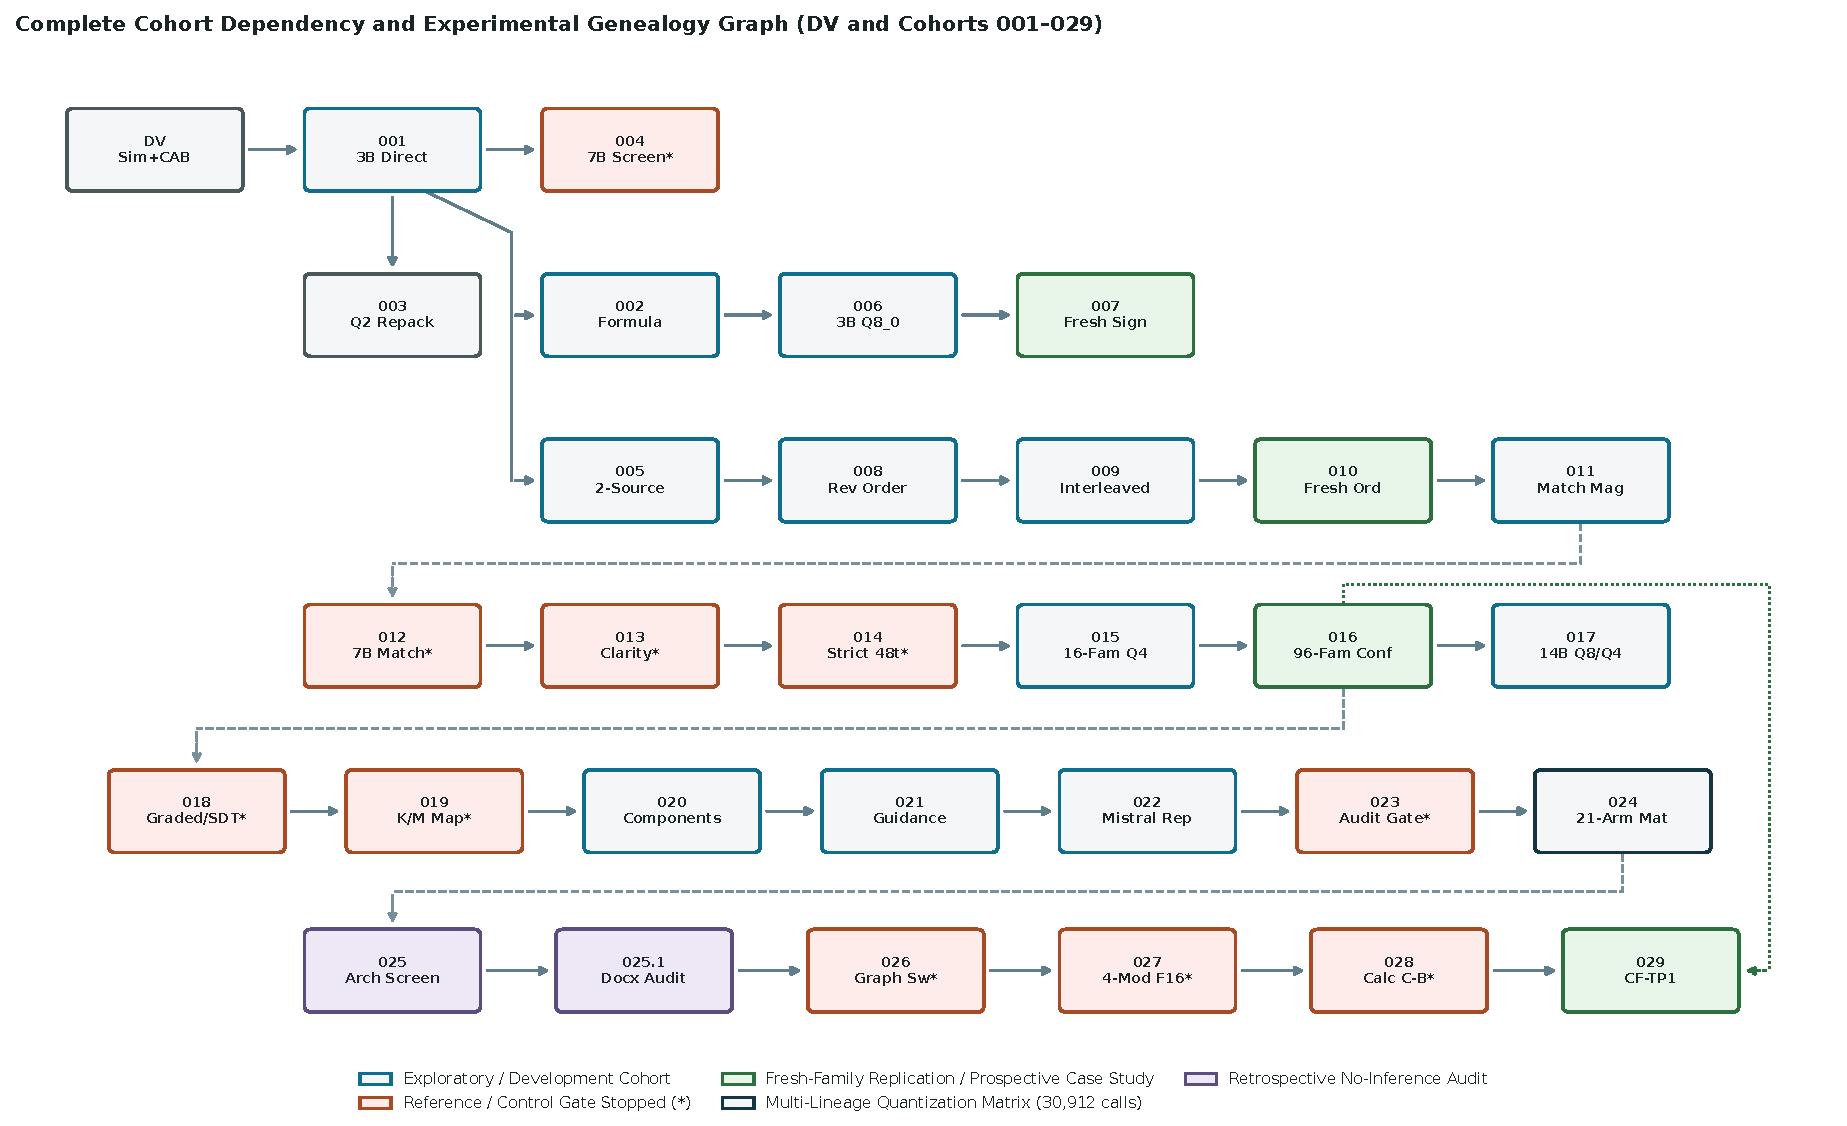
\includegraphics[width=\textwidth]{figures/fig03_cohort_dependency_graph.pdf}
  \caption{Complete cohort dependency graph from \texttt{design\_validation} through Cohort~029, showing how empirical falsifications, parser repairs, and failed reference gates drove each methodological transition.}
  \label{fig:cohort_dep}
\end{figure}

% =============================================================================
\section{Pre-LLM Suite: \texttt{design\_validation} --- Synthetic C/A/B Parameter Recovery}

\subsection*{1. Historical Context}
Following the October 28, 2026 literature scoping (\texttt{4e2fe4f}), the researchers needed to build the data-generation package (\texttt{causalfade/}) and verify that their planned statistical estimators could actually recover causal sensitivity ($C$), associative reliance ($A$), and response bias ($B$) before spending compute on local GGUF models.

\subsection*{2. Research Question}
Can an Expectation-Maximization (EM) solver accurately recover the parameters $(C, A, B)$ of a CNI-style multinomial processing tree across realistic per-cell sample sizes, and can goodness-of-fit deviance distinguish sequential tree processing from continuous logistic cue integration?

\subsection*{3. Hypothesis}
\textbf{Classification:} \emph{Exploratory synthetic validation (\texttt{H02}).} Prior to simulation, the researchers expected simplex EM estimation to recover $(C, A, B)$ reliably in interior parameter regimes and expected parametric bootstrap $G^2$ deviance tests to detect non-tree generating mechanisms.

\subsection*{4. Experimental Design}
\begin{itemize}
  \item \textbf{Independent Variables:} Six true parameter scenarios (interior, low-$C$, high-$C$ near boundary, high-$A$, extreme-$B$, null) crossed with three cell sample sizes $n_{\mathrm{cell}} \in \{50, 200, 1000\}$ ($18$ cells $\times 200$ Monte Carlo repetitions $= 3{,}600$ synthetic datasets), plus three structural model-misspecification regimes ($500$ bootstrap replicates each) and a $24$-family ($192$-prompt) baseline task fixture (\texttt{seed=20261101}).
  \item \textbf{Dependent Variables:} Parameter bias, RMSE, near-simplex-boundary rate, EM nonconvergence count, bootstrap $G^2$ $p$-values, and held-out log-loss.
  \item \textbf{Models \& Quantization:} None (pure NumPy \texttt{2.3.5} simulation; explicitly flagged in \texttt{manifest.json} as \texttt{"synthetic\_design\_validation\_not\_LLM\_results"}).
\end{itemize}

\subsection*{5. Mathematical Formulation}
Synthetic binomial counts $K_{TS} \sim \mathrm{Binomial}(n_{\mathrm{cell}}, p_{TS})$ were drawn across $(T,S) \in \{0,1\}^2$ under equation~\eqref{eq:cab_tree}, $p_{TS} = C T + (1-C)[A S + (1-A)B]$, and compared against logistic integration $p_{TS}^{\mathrm{log}} = \sigma(\beta_0 + \beta_T(2T-1) + \beta_S(2S-1))$ via likelihood-ratio deviance $G^2 = 2\sum_{T,S} \bigl[K_{TS}\ln(K_{TS}/\hat{\mu}_{TS}) + (n_{\mathrm{cell}}-K_{TS})\ln((n_{\mathrm{cell}}-K_{TS})/(n_{\mathrm{cell}}-\hat{\mu}_{TS}))\bigr]$.

\subsection*{6. Experimental Execution}
Executed deterministically on November 1, 2026 (commit \texttt{6ab18d2}) via \texttt{causalfade/cab\_tree.py} and \texttt{causalfade/generate.py}. Simultaneously, baseline deterministic policies (\texttt{exact:backdoor}, \texttt{exact:association}, \texttt{exact:random}, and $n=2{,}000$ sampled counterparts) were verified on the $192$-prompt synthetic fixture.

\subsection*{7. Results}
\emph{(Contemporaneously reported in \texttt{results/design\_validation/parameter\_recovery.json} and Figure~\ref{fig:cab_recovery}.)}
\begin{itemize}
  \item \textbf{Baseline Oracle Verification:} On the $192$-prompt fixture ($24$ families $\times 4$ $(T,S)$ cells $\times 2$ evidence modes), \texttt{backdoor} achieved $100.0\%$ accuracy ($0$ invalids), naive \texttt{association} achieved exactly $50.0\%$ ($100\%$ aligned, $0\%$ conflict), and random guessing scored $42.71\%$ (exact) and $50.0\%$ (sampled).
  \item \textbf{Parameter Recovery:} In the interior regime $(C=0.65, A=0.45, B=0.50)$, RMSE improved from $(0.0506, 0.1407, 0.1527)$ at $n_{\mathrm{cell}}=50$ to $(0.0252, 0.0703, 0.0699)$ at $n_{\mathrm{cell}}=200$ and $(0.0113, 0.0309, 0.0315)$ at $n_{\mathrm{cell}}=1000$. However, near the upper boundary ($C \to 1$), $(1-C) \to 0$ starved downstream branches of effective sample size, producing $16$ interval nonconvergences.
  \item \textbf{Observational Equivalence Discovery:} While asymmetric logistic data ($\beta_0 \neq 0$) was strongly rejected ($G^2 = 702.75$, $p_{\text{boot}} = 0.0020$), \emph{symmetric} logistic integration ($\beta_0 = 0$, generating cell probabilities $[0.0474, 0.5000, 0.5000, 0.9526]$) yielded $G^2 = 0.6876$ ($p_{\text{boot}} = 0.4331$) and virtually identical held-out log-loss ($0.4444$ tree vs.\ $0.4444$ logistic).
\end{itemize}

\subsection*{8. Interpretation at the Time}
Recorded in \texttt{VALIDATION\_REPORT.md}: $C/A/B$ trees can serve only as descriptive summaries if model fit passes, never as proof of sequential cognitive stages, and $n_{\mathrm{cell}}=16$--$50$ pilots will exhibit wide uncertainty on conditional parameters $A$ and $B$.

\subsection*{9. Retrospective Interpretation}
This pre-LLM audit prevented a major conceptual error that had appeared in prior LLM moral-psychology papers \citep{wuDeng2025counts}: recognizing symmetric logistic equivalence \emph{before} Cohort~001 meant the team was primed to check additivity ($p_{11}-p_{10}-p_{01}+p_{00}=0$) in Cohort~005 and abandon the tree cleanly when additivity failed.

\subsection*{10. Methodological Limitations}
The synthetic generator used a fixed confounding multiplier $k$, inadvertently making observational gaps $|\RD_{\mathrm{obs}}|$ larger in aligned cells ($57.10\pp$) than in conflict cells ($38.04\pp$)---an imbalance not noticed until Cohort~005 and repaired in Cohort~011.

\subsection*{11. Scientific Contribution}
\emph{Methodological refutation \& statistical improvement:} Proved 4-cell observational equivalence between CNI/$C/A/B$ trees and symmetric logistic cue integration, and validated the blind public/oracle data contract.

\subsection*{12. Transition to Subsequent Research}
Supplied the exact $16$-family development subset ($64$ exact-probability prompts) deployed in Cohort~001's first live LLM pilot.

\subsection*{13. Evidence and Reproducibility}
Artifacts: \texttt{results/design\_validation/VALIDATION\_REPORT.md}, \texttt{parameter\_recovery.json} (SHA-256 \texttt{4997af34...}), \texttt{public\_tasks.jsonl} (\texttt{ed4232a1...}), \texttt{oracle\_truth.jsonl} (\texttt{9a11f0fb...}); commit \texttt{6ab18d2}.

% =============================================================================
\section{Cohort 001: Direct Backdoor Causal Pilot on \texttt{Qwen2.5-3B}}

\subsection*{1. Historical Context}
With synthetic data generation validated and local \texttt{Qwen2.5-3B-Instruct} GGUF weights prepared on SSD (\texttt{F16}, \texttt{Q4\_K\_M}, \texttt{Q2\_K}), Cohort~001 executed the project's first live LLM experiment on November 10, 2026.

\subsection*{2. Research Question}
On exact 4-stratum confounded probability tables with an explicit causal graph ($Z\to X, Z\to Y, X\to Y$), what is \texttt{Qwen2.5-3B}'s baseline interventional accuracy and conflict penalty at \texttt{F16}, and how do \texttt{Q4\_K\_M} and \texttt{Q2\_K} alter performance?

\subsection*{3. Hypothesis}
\textbf{Classification:} \emph{Exploratory pilot of prospective hypothesis \texttt{H01}.} Expected \texttt{F16} to establish non-trivial causal competence and \texttt{Q2\_K} (and possibly \texttt{Q4\_K\_M}) to exhibit an inflated aligned-minus-conflict penalty.

\subsection*{4. Experimental Design}
\begin{itemize}
  \item \textbf{Arms:} \texttt{Qwen2.5-3B-Instruct} in \texttt{F16} (\texttt{run\_001\_f16}), \texttt{Q2\_K} (\texttt{run\_001\_q2\_k}), and \texttt{Q4\_K\_M} (\texttt{run\_001\_q4\_k\_m}).
  \item \textbf{Sample:} $16$ development families $\times 4$ $(T,S)$ cells $= 64$ exact-probability prompts per arm ($192$ total requests).
  \item \textbf{Execution Settings:} \texttt{temperature=0.0}, \texttt{max\_tokens=160}, \texttt{threads=8}, \texttt{seed=20261110}.
  \item \textbf{Required Output:} JSON with keys \texttt{ate\_estimate}, \texttt{activate}, and \texttt{adjustment\_set}.
\end{itemize}

\subsection*{5. Mathematical Formulation}
Each prompt supplied $\Prob(Y=1\mid X=x, Z=z)$ and joint cell masses $\Prob(Z=z, X=x)$ with target $\Prob(Z=0)=\Prob(Z=1)=0.5$, requiring equation~\eqref{eq:backdoor}: $\ATE = 0.5[\Prob(Y=1\mid 1,0)-\Prob(Y=1\mid 0,0)] + 0.5[\Prob(Y=1\mid 1,1)-\Prob(Y=1\mid 0,1)]$ and optimal action $\mathbb{I}(\ATE > 0)$.

\subsection*{6. Experimental Execution}
All $192$ HTTP completions succeeded and were logged to \texttt{raw\_responses.jsonl}. Representative verbatim outputs on task \texttt{6e39f6152120c3d91bc7} reveal what happened immediately:
\begin{lstlisting}
# F16 (finish_reason="stop", parse_status="invalid_json_or_response"):
```json
{
    "ate_estimate": -0.052625,
    "activate": 1,
    "adjustment_set": ["X"]
}
```
# Q2_K (finish_reason="length", 160 tokens):
\n"):\443333"4333 the"4663\n4\"6)\,\n\n\n"",...
\end{lstlisting}

\subsection*{7. Results}
\emph{(Contemporaneous statistics from \texttt{experiments/cohort\_001/summary.md} and \texttt{f16\_vs\_q4\_k\_m.json}.)}
\begin{itemize}
  \item \textbf{Strict Bare-JSON Scoring:} $0/64$ ($0.0\%$) valid across all three arms! Both \texttt{F16} and \texttt{Q4\_K\_M} wrapped all $64$ responses in Markdown \texttt{```json} fences (note: across the broader 192-item preliminary check noted in audit logs, strict bare JSON without fence stripping failed almost universally).
  \item \textbf{Single-Fence-Stripped Diagnostic Scoring:}
    \begin{itemize}
      \item \texttt{F16}: $64/64$ parseable; $33/64$ ($51.56\%$) action accuracy ($17/32$ aligned, $16/32$ conflict); recommended \texttt{activate=1} on \textbf{$63/64$ items} ($98.4\%$)! Valid adjustment set \texttt{["Z"]}: \textbf{$0/64$} (routinely emitted \texttt{["X"]} or \texttt{["Z","X"]}). Numeric ATE sign accuracy: $34/64$ ($53.1\%$, MAE $0.246$).
      \item \texttt{Q4\_K\_M}: $64/64$ parseable; $34/64$ ($53.13\%$) action accuracy; \texttt{activate=1} on $62/64$ items; numeric ATE sign accuracy: $35/64$ ($54.7\%$, MAE $0.222$).
      \item \texttt{Q2\_K}: $0/64$ parseable ($64/64$ hit the 160-token cap in repetitive digit/punctuation loops). \texttt{tokenizer\_metadata\_audit.json} confirmed GGUF tokenizer metadata matched \texttt{F16} byte-for-byte.
    \end{itemize}
\end{itemize}

\subsection*{8. Interpretation at the Time}
Cohort~001 exposed three immediate blockers: (1) strict bare-JSON parsing rejected normal chat-tuned Markdown fences; (2) \texttt{3B Q2\_K} was completely unusable due to generative looping; and (3) even \texttt{3B F16} lacked reference competence ($33/64 \approx$ chance, $63/64$ \texttt{activate=1}, $0/64$ adjustment set, and frequent disagreement between negative \texttt{ate\_estimate: -0.052625} and \texttt{activate: 1}!).

\subsection*{9. Retrospective Interpretation}
Look closely at the verbatim \texttt{F16} response above: on its very first item in the entire project, \texttt{Qwen2.5-3B F16} estimated a \emph{negative} treatment effect (\texttt{-0.052625}) and simultaneously set \texttt{"activate": 1}! Every major theme of CausalFade---parser artifacts, action-prior dominance, numeric-action dissociation, and reference-model incompetence---was already visible in embryo in Cohort~001.

\subsection*{10. Methodological Limitations}
Small 3B capacity, 3-field output complexity, Markdown fence mismatch, and reuse of $16$ development families.

\subsection*{11. Scientific Contribution}
\emph{Infrastructure discovery \& negative baseline finding:} Motivated fence-aware secondary diagnostics (\texttt{D03}), proved \texttt{3B Q2\_K} token-loop collapse, and uncovered extreme \texttt{activate=1} bias alongside numeric-action inconsistency.

\subsection*{12. Transition to Subsequent Research}
Spawned three parallel diagnostic branches on the same day: Cohort~002 (supplying the explicit arithmetic formula to separate causal identification from calculation), Cohort~003 (testing whether \texttt{llama-server} CPU repacking caused \texttt{Q2\_K}'s collapse), and Cohort~004 (testing whether scaling to \texttt{Qwen2.5-7B F16} solved the direct backdoor task).

\subsection*{13. Evidence and Reproducibility}
Artifacts: \texttt{experiments/cohort\_001/summary.md}, \texttt{f16\_vs\_q2\_k.json}, \texttt{f16\_vs\_q4\_k\_m.json}, \texttt{tokenizer\_metadata\_audit.json}, \texttt{run\_001\_*/raw\_responses.jsonl}; commit \texttt{0333c67}.

% =============================================================================
\section{Cohort 002: Formula-Given Arithmetic Control on \texttt{Qwen2.5-3B}}

\subsection*{1. Historical Context}
In Cohort~001, \texttt{Qwen2.5-3B} failed both causal adjustment-set selection ($0/64$) and numerical ATE estimation ($34/64$ sign accuracy). Before blaming ``causal reasoning,'' the researchers asked whether the 3B model could even compute the backdoor weighted average when handed the exact formula explicitly.

\subsection*{2. Research Question}
If the causal graph narrative is replaced by the explicit algebraic standardization formula on the exact same $64$ numerical tables, do \texttt{F16} and \texttt{Q4\_K\_M} compute accurate ATE signs and flip their binary actions accordingly?

\subsection*{3. Hypothesis}
\textbf{Classification:} \emph{Exploratory control (\texttt{H04}).} Expected explicit formula provision to boost both numeric ATE estimation and explicit action accuracy.

\subsection*{4. Experimental Design}
\begin{itemize}
  \item \textbf{Arms:} \texttt{Qwen2.5-3B-Instruct} \texttt{F16} (\texttt{run\_001\_f16}) and \texttt{Q4\_K\_M} (\texttt{run\_002\_q4\_k\_m}).
  \item \textbf{Sample:} Identical $16$ families ($64$ tables/arm, $128$ total requests) and task IDs from Cohort~001, replacing causal story prose with the explicit weighted-difference formula while keeping the 3-key JSON contract.
\end{itemize}

\subsection*{5. Mathematical Formulation}
Direct evaluation of $\hat{\tau} = 0.5[p_{10} - p_{00}] + 0.5[p_{11} - p_{01}]$ from supplied stratum probabilities $p_{xz} = \Prob(Y=1\mid X=x, Z=z)$, compared on (i) explicit binary decision $\hat{a} \in \{0,1\}$, (ii) numeric sign accuracy $\mathbb{I}(\sign(\hat{\tau}) = \sign(\tau))$, and (iii) internal disagreement $\mathbb{I}(\hat{a} \neq \mathbb{I}(\hat{\tau} > 0))$.

\subsection*{6. Experimental Execution}
Completed November 10, 2026 (\texttt{temperature=0.0}, \texttt{max\_tokens=160}). All $128$ responses stopped normally inside single \texttt{```json} fences ($0/64$ strict bare JSON; $64/64$ fence-valid).

\subsection*{7. Results}
\emph{(Contemporaneous metrics from \texttt{experiments/cohort\_002/summary.md} and Figure~\ref{fig:control_arch}A.)}
\begin{itemize}
  \item \textbf{Numeric ATE Sign Accuracy Surged---and Diverged by Precision:} \texttt{F16} jumped from $34/64$ (Cohort~001) to \textbf{$61/64$ ($95.31\%$)} (MAE dropping from $0.246$ to $0.062$), whereas \texttt{Q4\_K\_M} rose only from $35/64$ to \textbf{$45/64$ ($70.31\%$)} (MAE $0.081$). Post-hoc sign-derived policy accuracy differed by \textbf{$-25.00\pp$} under \texttt{Q4\_K\_M} vs.\ \texttt{F16} (paired 16-family percentile 95\% CI $[-37.50, -10.94]\pp$), spread evenly across aligned ($-7$ items) and conflict ($-9$ items; conflict-penalty shift $+6.25\pp$, CI $[-9.38, +21.88]\pp$).
  \item \textbf{Complete Polarity Flip in Explicit Binary Actions:} Whereas Cohort~001 \texttt{F16} chose \texttt{activate=1} on $63/64$ items, Cohort~002 \texttt{F16} chose \texttt{activate=1} on \textbf{$0/64$ items} ($100\%$ \texttt{activate=0}, scoring $32/64 = 50.0\%$)! \texttt{Q4\_K\_M} chose \texttt{activate=1} on $3/64$ items ($35/64 = 54.69\%$). Consequently, explicit actions \emph{disagreed with the model's own numeric ATE sign} on $29/64$ (\texttt{F16}) and $48/64$ (\texttt{Q4\_K\_M}) items!
\end{itemize}

\begin{figure}[htbp]
  \centering
  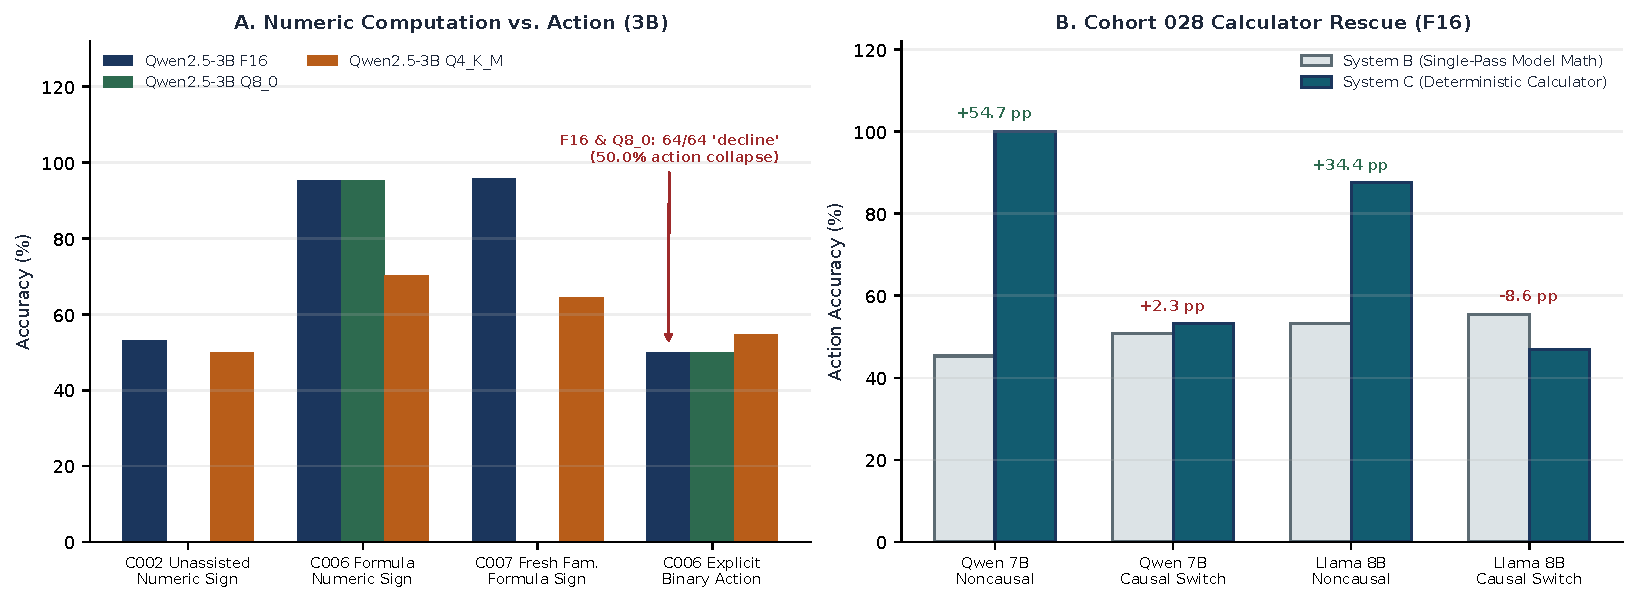
\includegraphics[width=\textwidth]{figures/fig12_experimental_control_architecture.pdf}
  \caption{Control-task dissociations across CausalFade: (A) Numeric ATE sign accuracy vs.\ explicit binary action collapse across Cohorts~002, 006, and 007 on \texttt{Qwen2.5-3B}; (B) Cohort~028 deterministic calculator rescue on noncausal named-rule tasks vs.\ null effect on causal graph-switch tasks.}
  \label{fig:control_arch}
\end{figure}

\subsection*{8. Interpretation at the Time}
Documented in \texttt{experiments/cohort\_002/summary.md}: (1) \texttt{3B F16} \emph{can} execute backdoor arithmetic ($61/64$) when told which formula to compute, proving Cohort~001's failure was an identification/formulation bottleneck rather than raw inability to add four numbers; (2) \texttt{3B Q4\_K\_M} exhibits a candidate $-25\pp$ arithmetic-execution deficit under this scaffold (not a selective causal-conflict deficit); and (3) explicit binary decisions in 3-key JSON are completely decoupled from numeric estimates and flip wildly ($63/64 \to 0/64$ \texttt{activate}) with prompt wording.

\subsection*{9. Retrospective Interpretation}
Cohort~002 produced the single strongest genuine quantization difference in the entire CausalFade archive ($-25\pp$, later replicated at $-31.25\pp$ in Cohort~007)---and crucially, it occurred on \emph{explicit formula execution} equally across aligned and conflict cells, confirming \citet{li2025meets} (low-bit arithmetic degradation) rather than \texttt{H01} (selective causal confounding fallback).

\subsection*{10. Methodological Limitations}
Reused Cohort~001's 16 development families; sign scoring was formulated post-hoc after observing the $0/64$ action collapse; Markdown fences persisted.

\subsection*{11. Scientific Contribution}
\emph{Positive empirical finding (arithmetic quantization drop) \& benchmark artifact discovery (numeric-vs.-action dissociation).}

\subsection*{12. Transition to Subsequent Research}
Prompted Cohort~006 (\texttt{Q8\_0} intermediate precision check) and Cohort~007 (prospective fresh-family replication of the formula-sign deficit).

\subsection*{13. Evidence and Reproducibility}
Artifacts: \texttt{experiments/cohort\_002/summary.md}, \texttt{f16\_vs\_q4\_k\_m\_formula.json}, \texttt{estimate\_sign\_policy\_sensitivity.json}; commit \texttt{f2b2cb1}.

% =============================================================================
\section{Cohort 003: \texttt{llama.cpp} CPU Weight-Repacking Diagnostic on \texttt{3B Q2\_K}}

\subsection*{1. Historical Context}
In Cohort~001, \texttt{Qwen2.5-3B Q2\_K} emitted $64/64$ length-capped gibberish loops. Before declaring 2-bit compression unusable at 3B scale, good systems hygiene required testing whether \texttt{llama-server}'s runtime CPU tensor repacking kernel corrupted \texttt{Q2\_K} dequantization on the host processor.

\subsection*{2. Research Question}
Does passing \texttt{--no-repack} to \texttt{llama-server} eliminate or reduce \texttt{Qwen2.5-3B Q2\_K}'s token-looping collapse?

\subsection*{3. Hypothesis}
\textbf{Classification:} \emph{Technical diagnostic (\texttt{H03}).} Tested whether runtime SIMD weight repacking caused the \texttt{Q2\_K} failure.

\subsection*{4. Experimental Design}
Two arms on \texttt{qwen2.5-3b-instruct-q2\_k.gguf}: \texttt{run\_001\_default} (default CPU repacking) vs.\ \texttt{run\_002\_no\_repack} (\texttt{--no-repack}), evaluated on the first $4$ development families ($16$ exact prompts/arm, $32$ total requests; \texttt{max\_tokens=160}, \texttt{temperature=0.0}).

\subsection*{5. Mathematical Formulation}
Floating-point matrix-vector multiplication is non-associative in finite SIMD registers; changing memory layout (\texttt{repack} vs.\ \texttt{--no-repack}) alters summation order at machine epsilon $\mathcal{O}(2^{-24})$, which can diverge chaotically once argmax ties occur in an unstable low-bit trajectory.

\subsection*{6. Experimental Execution}
Completed November 10, 2026 (commit \texttt{941cf7e}). Compare verbatim outputs on identical task \texttt{3e459f5e3dcade7fc172}:
\begin{lstlisting}
# run_001_default (length-capped):
\n"43)366323\n43\"333364333333643333334333333333...
# run_002_no_repack (length-capped):
\n"43)366323\n43)\n436363663663663366333646363333...
\end{lstlisting}

\subsection*{7. Results}
Both \texttt{run\_001\_default} and \texttt{run\_002\_no\_repack} scored \textbf{$0/16$ valid} ($0.0\%$) and hit \texttt{finish\_reason="length"} on \textbf{$16/16$ items} ($100\%$). Interestingly, exact output strings diverged after the first $\sim 12$ characters on $16/16$ items (confirming floating-point reduction-order sensitivity), but neither kernel produced coherent English or JSON.

\subsection*{8. Interpretation at the Time}
\texttt{3B Q2\_K} collapse is intrinsic to uncalibrated 2-bit weight quantization of \texttt{Qwen2.5-3B-Instruct}, not a \texttt{llama.cpp} CPU repacking bug.

\subsection*{9. Retrospective Interpretation}
A textbook systems control: had the team skipped Cohort~003, a skeptical reviewer could reasonably have blamed SIMD kernel bugs for low-bit failure. Later, Cohort~024 showed that at $7\text{B}$--$8\text{B}$ scale, \texttt{Q2\_K} achieved $99.7\%$--$100\%$ strict JSON validity across Qwen, Mistral, and Llama, confirming that severe syntactic collapse at \texttt{Q2\_K} was specific to small 3B model capacity under uncalibrated PTQ \citep{alimaskina2026extreme}.

\subsection*{10. Methodological Limitations}
Tested one \texttt{Q2\_K} artifact built without an importance matrix (\texttt{imatrix}).

\subsection*{11. Scientific Contribution}
\emph{Infrastructure discovery:} Ruled out inference-engine repacking artifacts and justified retiring \texttt{3B Q2\_K}.

\subsection*{12. Transition to Subsequent Research}
Closed the \texttt{3B Q2\_K} investigation and shifted focus to \texttt{Q4\_K\_M}, \texttt{Q8\_0}, and larger 7B models.

\subsection*{13. Evidence and Reproducibility}
Artifacts: \texttt{experiments/cohort\_003/summary.md}, \texttt{repack\_comparison.json}, \texttt{run\_001\_default/}, \texttt{run\_002\_no\_repack/}; commit \texttt{941cf7e}.

% =============================================================================
\section{Cohort 004: \texttt{Qwen2.5-7B F16} Direct-Table Reference Competence Screen}

\subsection*{1. Historical Context}
Since \texttt{Qwen2.5-3B F16} scored at chance ($33/64$) and $0/64$ on adjustment sets in Cohort~001, the researchers introduced an explicit methodological rule (\texttt{D04}): \emph{before evaluating quantized arms on a new model or task, the unquantized \texttt{F16} reference must pass a pre-declared competence gate}. Cohort~004 applied this gate to \texttt{Qwen2.5-7B-Instruct F16}.

\subsection*{2. Research Question}
Does scaling parameter count from $3\text{B}$ to $7\text{B}$ at \texttt{F16} enable reliable direct causal decisions ($\ge 22/32$ overall accuracy) on the Cohort~001 4-stratum backdoor table prompt?

\subsection*{3. Hypothesis}
\textbf{Classification:} \emph{Documented prospective feasibility gate.} Pre-specified threshold: overall fence-stripped accuracy $\ge 22/32$ ($68.75\%$) required before running \texttt{7B Q2\_K} or \texttt{7B Q4\_K\_M}.

\subsection*{4. Experimental Design}
Single arm (\texttt{Qwen2.5-7B-Instruct F16}) on $8$ development families ($32$ exact-probability prompts: $16$ aligned, $16$ conflict; \texttt{max\_tokens=160}, \texttt{temperature=0.0}).

\subsection*{5. Mathematical Formulation}
Identical 4-stratum backdoor adjustment target~\eqref{eq:backdoor} as Cohort~001.

\subsection*{6. Experimental Execution}
Completed November 10, 2026 (commit \texttt{01c7590}); all $32$ responses finished normally inside \texttt{```json} fences.

\subsection*{7. Results}
\begin{itemize}
  \item \textbf{Graph Identification Improved Dramatically:} Unlike \texttt{3B F16} ($0/64$), \texttt{7B F16} output the exact valid backdoor adjustment set \texttt{["Z"]} on \textbf{$32/32$ items ($100\%$)}!
  \item \textbf{Action Gate Failed Due to \texttt{activate=1} Bias:} Despite naming \texttt{["Z"]} correctly on every item, \texttt{7B F16} recommended \texttt{activate=1} on \textbf{$31/32$ items ($96.9\%$)}, yielding \textbf{$17/32$ ($53.13\%$)} overall action accuracy ($8/16$ aligned, $9/16$ conflict)---failing the $\ge 22/32$ gate. Strict bare-JSON accuracy was $0/32$.
\end{itemize}

\subsection*{8. Interpretation at the Time}
Scaling to 7B solved symbolic adjustment-set naming (\texttt{["Z"]} $32/32$) but left end-to-end table standardization and binary decision-making trapped in a $97\%$ \texttt{activate=1} default policy. Per the pre-declared gate, quantized 7B runs were withheld.

\subsection*{9. Retrospective Interpretation}
Cohort~004 provided the first glimpse of a pattern that recurred in Cohorts~021 and 027: \emph{declarative causal graph knowledge (\texttt{["Z"]} = 100\%) does not mean a language model applies that graph when computing an action}.

\subsection*{10. Methodological Limitations}
Small $8$-family ($32$-item) screen; bundled multi-step arithmetic with causal identification in one pass without scratchpad tokens.

\subsection*{11. Scientific Contribution}
\emph{Negative result \& methodological gate enforcement:} Demonstrated declarative-vs.-procedural causal dissociation at 7B and enforced the reference-competence gate for the first time.

\subsection*{12. Transition to Subsequent Research}
Because direct 4-cell backdoor arithmetic blocked both 3B and 7B references, Cohort~005 simplified the task by pre-computing the interventional and historical summary rates directly into a two-study source-selection problem.

\subsection*{13. Evidence and Reproducibility}
Artifacts: \texttt{experiments/cohort\_004/summary.md}, \texttt{run\_001\_f16/results.json}, \texttt{raw\_responses.jsonl}; commit \texttt{01c7590}.
